\documentclass[a4paper,fleqn,twoside,12pt]{article}

%%%%%%%%%%%%%%%%%%%%


\usepackage[]{geometry}
\usepackage[latin1]{inputenc}
\usepackage[UKenglish]{babel}
\usepackage[UKenglish]{isodate}
\usepackage{amsmath}
\usepackage{amsfonts}
\usepackage{amssymb}
\usepackage{amsthm}
\usepackage{graphicx}
\usepackage{chngpage}
\usepackage{calc}
\PassOptionsToPackage{hyphens}{url}
\usepackage{hyperref}
\usepackage[nameinlink]{cleveref}
\usepackage{fancyhdr}
\usepackage{titletoc}
\usepackage[explicit]{titlesec}
\usepackage[]{biblatex}
\usepackage[dvipsnames]{xcolor}
\usepackage[sc]{mathpazo}
\linespread{1.05}
\usepackage[T1]{fontenc}
\usepackage{minted}
\usepackage{listings}

\addbibresource{common/bibliography.bib}

\hypersetup{
	colorlinks=true,
	linkcolor=black,
	urlcolor=black,
	citecolor=black
}

\setlength{\parindent}{0mm}
\setlength{\parskip}{\medskipamount}
\renewcommand\baselinestretch{1.2}

\cleanlookdateon

\makeatletter
\newcommand{\@assignment}[0]{Assignment}
\newcommand{\assignment}[1]{\renewcommand{\@assignment}{#1}}
\newcommand{\@supervisor}[0]{}
\newcommand{\supervisor}[1]{\renewcommand{\@supervisor}{#1}}
\newcommand{\@yearofstudy}[0]{}
\newcommand{\yearofstudy}[1]{\renewcommand{\@yearofstudy}{#1}}
\makeatletter

\newtoggle{IsDissertation}

%%%%%%%%%%%%%%%%%%%%%%%%%%%%%%%%%%%%%%%%%%%%%%%%%%%%%%%%%%%%%%%%%%%%%%%%%%%%%%%
%% Project-specific configuration
%%%%%%%%%%%%%%%%%%%%%%%%%%%%%%%%%%%%%%%%%%%%%%%%%%%%%%%%%%%%%%%%%%%%%%%%%%%%%%%

\author{Noah Hollowell}
\title{Visual RISC V Simulator}
% \supervisor{Your supervisor's name}
% \yearofstudy{3\textsuperscript{rd}}

%%%%%%%%%%%%%%%%%%%%%%%%%%%%%%%%%%%%%%%%%%%%%%%%%%%%%%%%%%%%%%%%%%%%%%%%%%%%%%%


\assignment{Progress report}

%%%%%%%%%%%%%%%%%%%%

\pagestyle{plain}
\renewcommand{\headrulewidth}{0.0pt}

\makeatletter
\fancypagestyle{plain}{
	\fancyhf{}
	\fancyhead[LE]{\thepage}
	\fancyhead[RE]{\textit{\@author}}
	\fancyhead[RO]{\thepage}
	\fancyhead[LO]{\textit{\@title}}
}
\makeatother

%%%%%%%%%%%%%%%%%%%%

\begin{document}

\input{../common/titlepage.tex}

\pagestyle{plain}

\section{Introduction}
Within the understanding of how a modern processor works we often look into the underlying instructions and physical operations it performs. However, often being able to visualise
those are far more beneficial to our understanding than simply emulating the physical code to produce a result.
\\\\
RISC-V is a new open source instruction set that has numerous emulators available online with a varying degree of visual elements.
These all lack the ability to fully visualise the internal operations during each instruction execution. Thus, the aim is to produce a fully fledged RISC-V simulator that not only emulates RISC-V code but also visually demonstrates the flow of data during execution all the way down to data moving across the processor to their respective components updating in real-time.
\section{Objectives}
So far, the project has progressed along nicely, with a few objectives now being complete, or . Later objectives remain relatively unchanged.

Over the past 8 weeks the following objectives have been completed:
\begin{itemize}
    \item Emulation of the base instruction set: RV32I \cite{risc_spec}, as per the RISC-V specification,
    \item Partial lexical and semantic analysis of code
    \item The start of the visualisation process for animating instructions including:
        \begin{itemize}
            \item Speed control,
            \item Manipulation of multiple values simultaneously.
        \end{itemize}
\end{itemize}

All other objectives below remain in a to-do state with the visualisation objectives currently holding the most importance to produce the desired minimval viable product as mentioned in the specification \cite{hollowell_2022_visual}: (New additions/changes are in \textit{italics})



\begin{enumerate}
    \item \textbf{(M)} A lexical analysis of inputted RISC-V code,
    \item \textbf{(S)} A semantic analysis of inputted RISC-V code,
    \item \textbf{(C)} \textit{Loop control via labelled functions}
    \item \textbf{(S)} Emulation of the "Standard Extension for Integer Multiplication and Division" instruction set,
    \item \textbf{(A)} Emulation of the "Standard Extension for Single-Precision Floating-Point" instruction set
    \item \textbf{(M)} A visualisation of the processors register set,
    \item \textbf{(M)} A visualisation of the memory holding both the instructions and data or just data,
    \item \textbf{(M)} A comprehensive system allowing for the display of data moving around the processor including:
    \begin{enumerate}
        \item \textbf{(M)} Numerical data moving from memory to other components and vice-versa,
        \item \textbf{(S)} Addressing requests,
        \item \textbf{(C)} Manipulation of multiple values simultaneously to simulate the effect of processor operations (e.g. addition, subtraction, shifts, etc),
    \end{enumerate}
    \item \textbf{(C)} Control \textit{the} steps of the simulation,
\end{enumerate}

To further help with development objectives have been extended to make use of the MoSCoW prioritisation method \cite{business_2022_chapter} (Must, Should, Could, Would) and have prefixed each objective with the respective capital.

Furthermore, the allocation of priorities matches with our timetable, in which the majority of \textbf{Must} items are due to be finished by the end of this term, with items such as 4. coming at the start of term 2. 

\section{Research}
Building a simulator for a instruction set from the ground up is no easy task. There are multiple ways to approach building both the emulation and visualisation parts of the simulator. With regards to the visualisation, after researching more into JavaFX \cite{sunmicrosystems_2022_javafx} we determined it to be a suitable choice after further experimentation into its abilities and how they would fit the the projects needs. A suitable fail-safe was also determined in the form of a web-based interface due to having an extensive history of web development and design.
\\\\
Research is focused on understanding the RISC-V RV32I \cite{risc_spec} instruction set and how each instruction individually operates. RISC provides an open-source reference card \cite{riscv_greencard} which provides information about each instruction including its operands and instruction type, which when coupled with the RISC-V specification \cite{risc_spec} provides comprehensive coverage of exactly how to implement each instruction according to the specification.
\\\\
In order to develop the visual end of the project research was done into existing solutions. A previous solution is Cornell's Online RISC-V Interpreter \cite{cornelluniversity_riscv}, which provides a comprehensive interface to show of registers  and memory as instructions execute either instantly, or in a stepped format. However, it lacks any form of animated view of a processor, which this project aims to build upon. It is also invaluable to have a robust comparison available to cross-reference instruction operations and devise working tests, or than purely using the RISC-V specification. Another useful system is LittleManComputer \cite{higginson_2014_little}. It is a simple instructional model of a computer, with a limited instruction set. However, unlike Cornell's it does display the movement of data around the processor, providing a base idea for how the project can animate the flow of data in a clear and comprehensive manner.


\section{Progress}
The project is currently in a very healthy state, with it being on-track to complete the minimal viable product for, or just after the start of the Christmas break.
\\\\
The project has been split up into two distinct sections: \textbf{Emulation} and \textbf{Visualisation}. This decision was made to allow decoupled development, providing the benefit of working exclusively on emulation for the first 5 weeks to ensure the core of the project is stable, reliable and robust. Only then, can work start to build upon the visual aspects which require the core to build upon its functionality into a fully fledged application whilst still being able to be developed independently in terms of GUI design and layout.
\subsection{Emulation}
Core to emulating RISC-V is its set of 32 unique 32-bit registers. These are core to performing operations on values during execution without having to constantly move data to-and-from memory.
\subsubsection{Registers}
Registers are implemented as a Map relating each registers name and alternate name to a \texttt{Register} instance that holds it value. For easy access each Register provides 3 ways to read out the data: As binary, as hexadecimal and as denary. Instead of writing 3 write methods directly on the register the decision was to have 3 write methods in the \texttt{RegisterSet}, a class manager that stores all 32 register instances. This class mainly handles reading and writing binary to the register with reading having 3 unique methods to retrieve data in specific formats (Binary, Hexadecimal and Denary) and 3 methods to write, which internally convert to binary and call the third write method that directly writes binary to the register.
\subsubsection{Memory}
Memory follows a similar suit to register, but deviates within that the memory consists of far more than 32 cells. As such an implementation very similar to the registers was used, except \texttt{MemoryCells} (instances that store the value in memory) are on the fly as they are needed. This helps keep the overhead down compared to pre-generating say 2000 memory cells and having to constantly search them for the required value. Further, with the usage of a Map to store memory cells, access time was also cut down significantly due to the constant O(1) search time compared to storing cells in a list which incurs a linear O(n) search times, which would become noticeable for massive memory operations within the program.

\subsubsection{Instructions}
A core part of the project is to be able to take in a user written set of instructions and convert them into operable instructions the the program can execute. Within this a very basic lexer has been produced, that allows us to convert written instructions into instances of the \texttt{Instruction} class.

The implementation of this relies heavily on a base abstract class (Listing \ref{lst:abstract_instr}) having an abstract \texttt{execute(InstructionOperands operands)} method that is then implemented for each instruction within its own implementation (Listing \ref{lst:add_impl}). 

An instance of \texttt{InstructionOperands} is then passed to the execute method, with \texttt{InstructionOperands} simply being an object holding up to three strings representing the operands of the current instruction.

To improve the usability and extend-ability of the project Instructions will automatically register themselves. Thus, any class that extends \texttt{Instruction} will be automatically found and loaded during run-time and then be available to be used in any user given program. This is performed by a library called Reflections \cite{ronmamo_2022_ronmamoreflections} which "scans and indexes your project's classpath metadata, allowing reverse transitive query of the type system on runtime" allowing us to perform the dynamic loading of classes during runtime. 
\\


\lstinputlisting[label={lst:abstract_instr},language=Java,breaklines=true,basicstyle=\tiny,caption={An abstract class representing the absolute minimum of an instruction that must be extended},captionpos=b]{abstract_instruction.java}

\lstinputlisting[label={lst:add_impl},language=Java,breaklines=true,basicstyle=\tiny,caption={An implementation of the abstract Instruction class for the ADD instruction.},captionpos=b]{add_impl.java}   

    




\subsubsection{Parsing \& Running}
Now that all the main pieces are ready progress can begin on building them up from a text input to being emulated.

Currently, a very basic parser operates by splitting an input line by line and then by splitting the lines. Instructions are expected to appear in multiple forms, mainly being of the form \texttt{OPCODE rd, rs1, rs2} (R type), in which \texttt{rd} \& \texttt{rs}\# are destination and target registers respectively. Deviation from this format occurs as RISC-V employs multiple instruction formats (\texttt{R, I, S, B, U}...)\cite{risc_spec} to allow for different size values to be entered. For example the \texttt{ADD} instruction is type R in which each operand is expected to be a register. Whereas for \texttt{ADDI} the last operand is a 12-bit immediate, taking a signed values between -2048 and 2047. To facilitate the occurrence further of instructions that take less operands the number of operands in each \texttt{Instruction}'s constructor must be specified with a default of 3. This way, the program runner can quickly check the amount of operands during parsing and reject any that have to many to to little for the respective instruction.
\\\\
A slight difficulty in parsing instructions is related to load and store instructions as these require a specific format to select memory registers to allow for more complex addressing. For all types, they follow the format \texttt{offset(register)}, which allows continuous data storage in memory (for example: an array) but also allows writing to any memory location (by using the zero register). However, within this the offset can be represented as both hexadecimal and denary so an method to determine which type is present in order to parse both and produce the same output at the end while being flexible and extendable in the future.

The solution was to encapsulate them into a \texttt{MemoryAddress} abstract class with two implementations (one for denary and one for hex) which both use a regex to parse out the offset and register and then combine them to return an integer memory location that the program can use. By doing this the memory controller can alter memory addressing without having to modify any of the memory read/writing code, and in turn the reading and writing code for memory only cares about receiving an instance of MemoryAddress, avoiding having duplicate methods just to allow denary or hex addressing.
\\\\
Finally, once all the instructions are parsed they are bundled up into a program instance which can then be executed. This is done in a iterative manner in which each instruction is executed, then the program counter is incremented (or jumped for branching), then the next instruction is fetched based on the program counters value and executed. This occurs until the program counter doesn't point to an instruction at which point execution has finished. At this point the memory and registers are printed to the console allowing us to verify operation and also see the values.

\subsection{Visualisation}
After Week 6 development switched from emulation to visualisation. This began with a rough mock-up (Figure \ref{fig:draft_layout}) of the interface, and then an actual implementation of the interface using JavaFX (Figure \ref{fig:javafx_layout})

\begin{figure}[H]
    \centering
    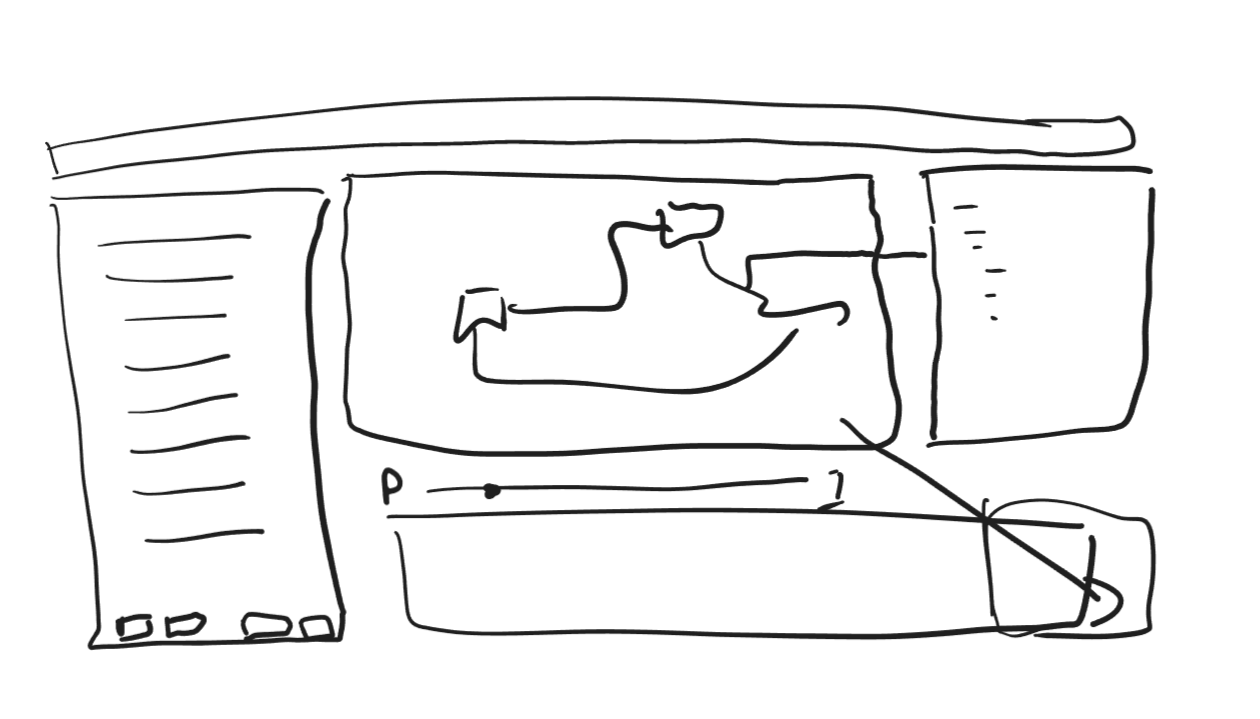
\includegraphics[scale=0.5]{progress-report/draft_layout.png}
    \caption{Draft Interface Layout}
    \label{fig:draft_layout}
\end{figure}
\begin{figure}[H]
    \centering
    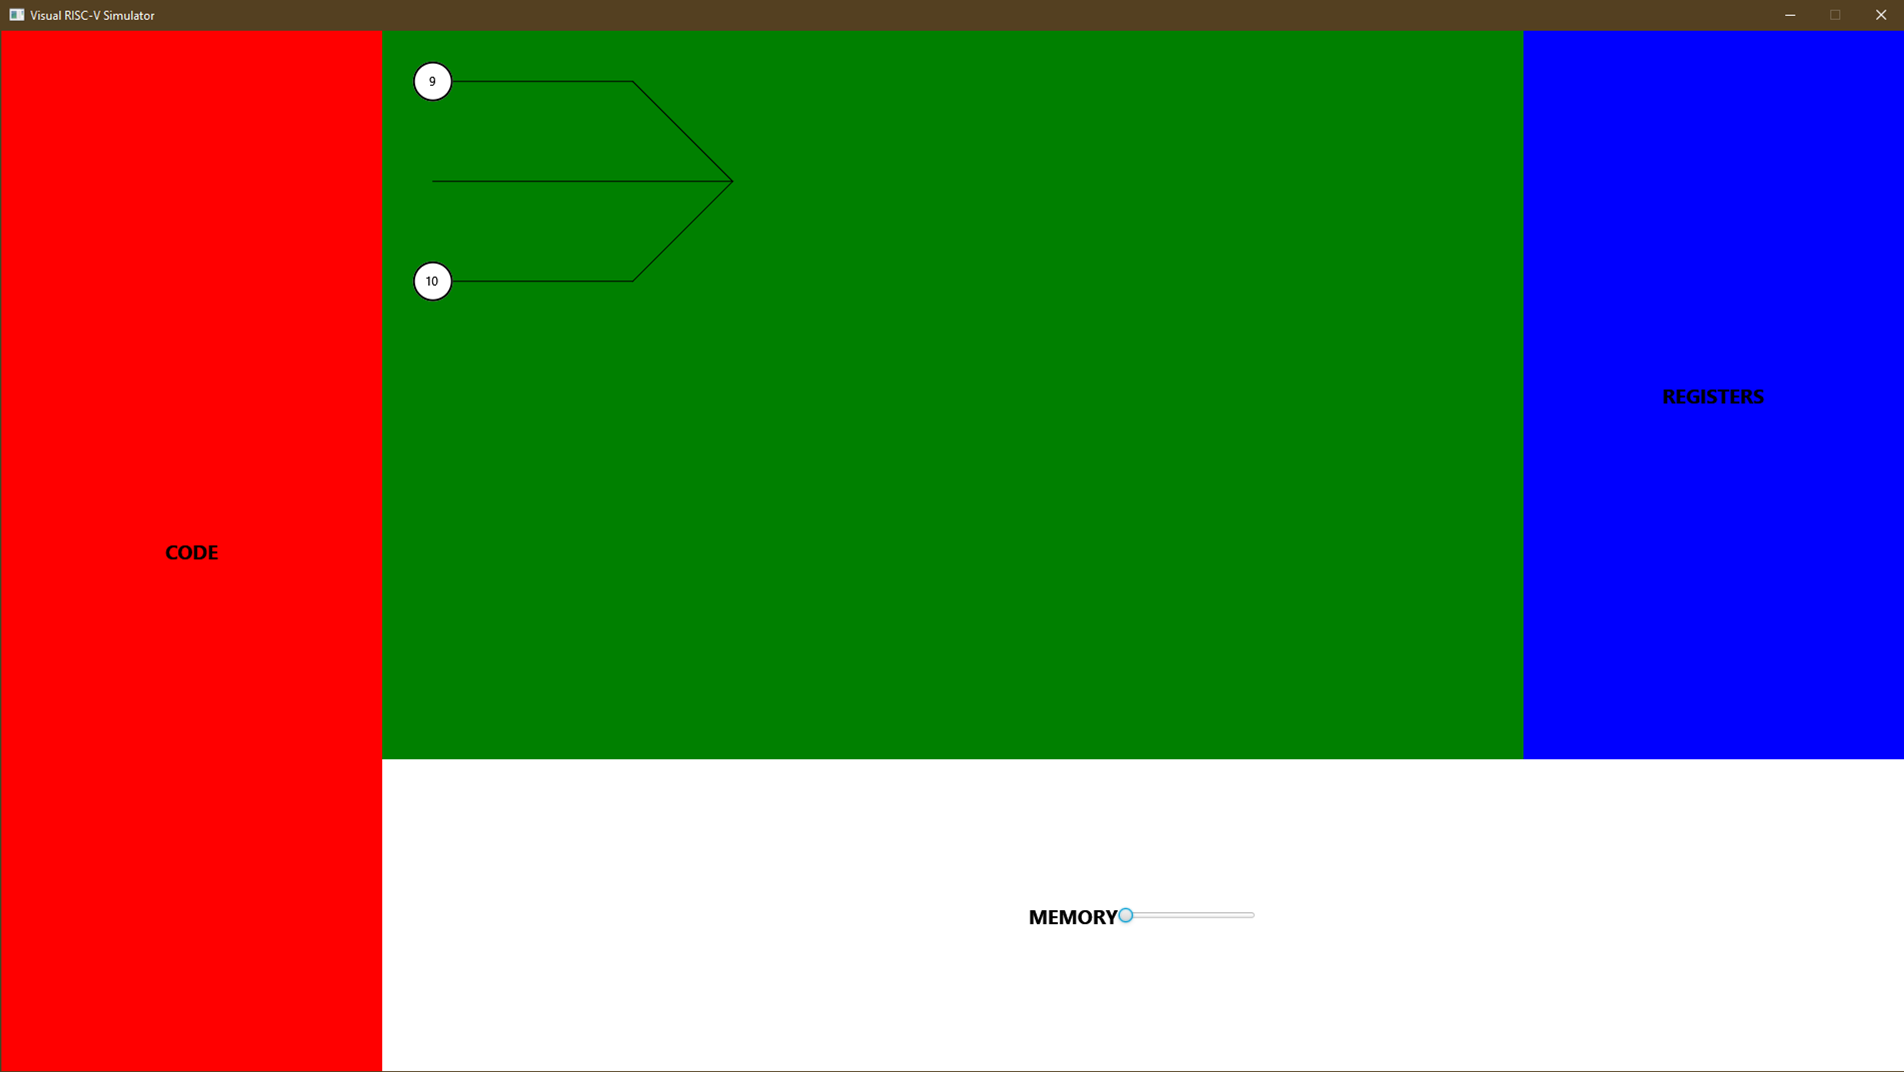
\includegraphics[scale=0.5]{progress-report/javafx_layout.png}
    \caption{Draft layout implemented in the application}
    \label{fig:javafx_layout}
\end{figure}

The design of the interface as seen in Figures \ref{fig:draft_layout} \& \ref{fig:javafx_layout} was determined based on usage of previous online interpreters such as LittleManComputer \cite{higginson_2014_little} and the Cornell RISC-V Interpreter \cite{cornelluniversity_riscv} which adopt a common layout of code input being on the left, and visual elements being on the right, centre and below. The layout prominently orients around the main central section in which the animated content will occur showing movement around the chip, with a larger section below to display memory as it read and written, with a smaller registers section on the right which will contain a fixed listing of the 32 registers, with active registers being highlighted.

After, development of the animation component began utilising JavaFX \cite{sunmicrosystems_2022_javafx}. JavaFX provides a path element to draw paths for us. However, implementing a custom version integrates better with the projects needs and removes unnecessary options that the path element provides. This, allows us to have a very simple pathing structure, whilst also being to directly animate on-top of the path without having to pull data out of the JavaFX path class and the process, instead having direct access to the nodes that makeup the path.

Within the custom paths, the \texttt{Line} object is used to draw paths onto the Scene (JavaFX denotes an open application window a Stage, that a Scene is then placed upon that contains our entire interface and its moving parts) as seen in Figure \ref{fig:javafx_layout}. Now, by utilising the \texttt{TranslateTransition} and \texttt{SequentialTransition} classes provided by JavaFX we can effectively animate data movement around the scene by utilising the path nodes to build up a transition per set of nodes to simulate following that path, using an overarching Sequential Transition per path to wrap all the transitions and play them in the correct order linearly to produce the visual effect of an element perfectly following the path.

To ensure consistency within animations an \texttt{Animator} class was developed, which encapsulates a set of stages that represent elements of an entire animation sequence. This starts with an abstract AnimatorStage class which provides two important methods:
\begin{itemize}
    \item \textbf{play}: Runs the given animation implementation
    \item \textbf{after}: Calls the parent Animator class to run the next stage if there is one
\end{itemize}

With this abstraction other stages can be implemented such as changing text and interpolating to a fixed point. 

As for our path animations, each calls \texttt{after()} once they have finished execution allowing the animator to call the next animation or call the animators finished callback, allowing us to run something after all the animation stages have finished.

Thanks to this level of abstraction, complex animations can be easily built up, traversing paths, moving to points or changing text at whim, with the option to easily add new animation options in the future with little hassle, with JavaFX taking care of transforming objects in the scene leaving us to just handle ordering and callbacks to ensure continuous operation.

\subsubsection{The problem}
Animating was not without is problems. JavaFX provides multiple ways to transition in its \verb|TranslateTransition| class, mainly \verb|setToX| and \verb|setByX| (and respective Y variants) which proved problematic due to a lack of documentation as to how these actually transform the given element on execution. 

After researching JavaFX's documentation and online resources, it was discovered that JavaFX tracks elements via coordinate positions, however when you apply a transition its base coordinates remain unchanged, but instead they are transformed by the transition provided. These transition coordinates then remain and are stacked upon by further transitions, meaning each transition is relative to the previous.

Originally using \verb|setToX| caused major issues as this would result in the transition playing, but not relative to the previous transition causing the element to fly off-screen and never follow the line. The solution was to use \verb|setByX| which moves the element relative to the previous transition producing the expected outcome of the element correctly following the path.

\section{Project Management}
Currently, the project has been on track following the set out timetable. However, I foresee that the project may run up to a week late with content due to the end of term being busy with Christmas events, competitions and moving back home for the break. Yet, this was factored in from the start with the Christmas break being intended as a buffer for any delays as well as small bits of extra work to be completed.

Supervisor meetings started as weekly meetings, but have drifted to being more fortnightly. This is mainly down to personal schedule changes and occasionally a lack of material to discuss due to parts of development yielding successful but rather dull material to cover.

Git and Github have remained for version control, making use of the builtin workflows to automate testing in a separate environment, which has helped lead to the discovery of unintended bugs. Branching has also been an indispensable to the project allowing separation of new features and content during development, allowing us to isolate development and merge complete features back together once complete. Also, as discussed in the specification DCS is being used as an alternate remote as an extra backup in-case anything were to happen to Github or my local machine. Thus, reducing the risk of total code loss which would be fatal to the project.

The Agile \cite{atlassian_2022_agile} methodology is still the main approach, with some plan driven aspects. However, the adopted methodology is mixture of agile and personal choices as rather than following a specific methodology. However, we have made good use of a backlog type system, in the form of a to-do list on Notion which has made tracking extra items to accomplish or fix on later dates much easier as-well as noting information about how systems should work.

Testing is still being fronted with test-driven development. However, this is problematic for visual elements due to the necessity for a physical person to need to watch the animations play to ensure they look correct which isn't possible in a test-drive scenario, thus visualisation tests are being performed in parallel with development.

\subsection{Risks}
No new risks have arisen during the term.

Because of the successful progress of the project the desired minimal viable product as set out in the specification is going to be completed for the Christmas break, giving a basis for feedback and further development.

Of our original risks, they remain unchanged, or resolved as mentioned above.

\subsection{Timetable}
The projects timetable given in the specification \cite{hollowell_2022_visual} remains unchanged.

\section{Legal, Social, Ethical \& Professional Issues}
Social, Ethical and Professional issues remain unchanged.

A decision to change the JDK used for the project incurs a slight legal change. The choice is due to how JavaFX is loaded into the project, and if it should be incorporated as part of the JDK or separately incorporated into the final application JAR manually. The choice of using a JDK with JavaFX already incorporated would mean using a more lax licensed JDK, which is beneficial to the project, with the majority of JDKs including JavaFX being . Alternatively, JavaFX can be incorporated manually and its own licensing will be followed along with Oracle's OpenJDK \cite{oraclecorporation_2022_openjdk} licensing.




\printbibliography

\end{document}